\section{Figures and Tables}
\label{chap:figures_tables}

This section contains all graphical representations and data tables referenced in the report.

% -----------------------------------------------------------------------------
% PLATE RESULTS
% -----------------------------------------------------------------------------
\subsection{Plate with Hole}

\begin{figure}[H]
    \centering
    \includegraphics[width=0.5\textwidth]{figures/plate_geometry.png}
    \caption{Geometry and boundary conditions of the plate with a hole.}
    \label{fig:plate_geom}
\end{figure}

\begin{figure}[H]
    \centering
    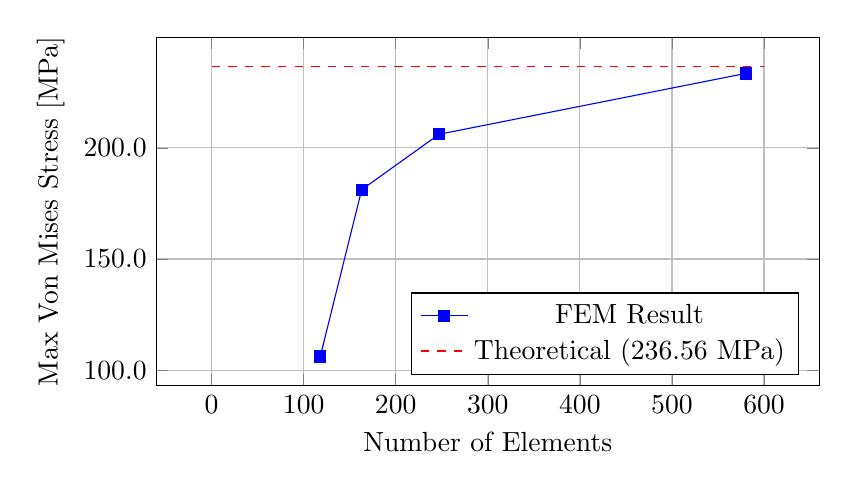
\begin{tikzpicture}
        \begin{axis}[
            width=10cm, height=6cm,
            xlabel={Number of Elements},
            ylabel={Max Von Mises Stress [MPa]},
            grid=major,
            legend pos=south east,
            y tick label style={/pgf/number format/.cd, fixed, fixed zerofill, precision=1}
        ]
        \addplot[color=blue, mark=square*] coordinates {
            (118, 106.129)
            (163, 181.176)
            (247, 206.095)
            (580, 233.478)
        };
        \addlegendentry{FEM Result}
        
        \addplot[color=red, dashed, domain=0:600] {236.56};
        \addlegendentry{Theoretical (236.56 MPa)}
        \end{axis}
    \end{tikzpicture}
    \caption{Convergence of maximum stress for the plate with hole.}
    \label{fig:plate_convergence}
\end{figure}

\begin{table}[H]
    \centering
    \small
    \caption{Stress convergence data for Plate with Hole.}
    \label{tab:plate_results}
    \begin{tabular}{lcc}
        \toprule
        \textbf{Mesh Quality} & \textbf{Nb. Elements} & \textbf{Max Stress [MPa]} \\
        \midrule
        Coarse      & 118 & 106.13 \\
        Moderate    & 163 & 181.18 \\
        Fine        & 247 & 206.10 \\
        Very Fine   & 580 & 233.48 \\
        \bottomrule
    \end{tabular}
\end{table}

% -----------------------------------------------------------------------------
% FRONT SPRING RESULTS
% -----------------------------------------------------------------------------
\subsection{Front Spring}

\begin{figure}[H]
    \centering
    \includegraphics[width=0.45\textwidth]{figures/spring_3coils_geom.png}
    \hfill
    \includegraphics[width=0.45\textwidth]{figures/spring_3coils_stress.png}
    \caption{Left: Geometric model of the 3-coil spring section. Right: Von Mises stress distribution under load.}
    \label{fig:front_spring_visu}
\end{figure}

\begin{figure}[H]
    \centering
    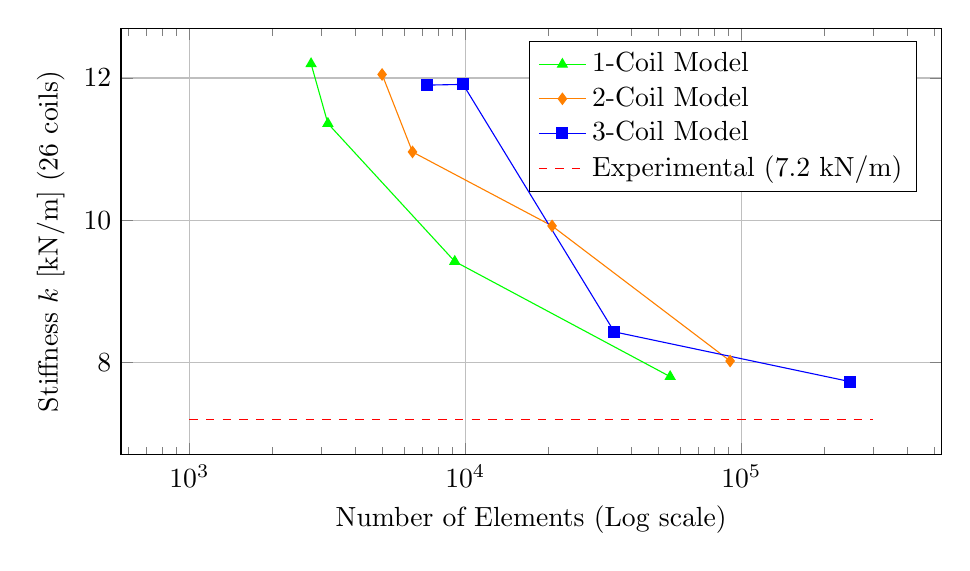
\begin{tikzpicture}
        \begin{axis}[
            width=12cm, height=7cm,
            xlabel={Number of Elements (Log scale)},
            ylabel={Stiffness $k$ [kN/m] (26 coils)},
            xmode=log,
            grid=major,
            legend pos=north east,
            legend style={cells={anchor=west}}
        ]
        % 1 Coil
        \addplot[color=green, mark=triangle*] coordinates {
            (2760, 12.2) (3176, 11.36) (9154, 9.42) (55218, 7.8)
        };
        \addlegendentry{1-Coil Model}
        
        % 2 Coils
        \addplot[color=orange, mark=diamond*] coordinates {
            (4992, 12.05) (6433, 10.96) (20613, 9.92) (91068, 8.02)
        };
        \addlegendentry{2-Coil Model}
        
        % 3 Coils
        \addplot[color=blue, mark=square*] coordinates {
            (7255, 11.90) (9813, 11.91) (34646, 8.43) (247630, 7.73)
        };
        \addlegendentry{3-Coil Model}
        
        % Experimental
        \addplot[color=red, dashed, domain=1000:300000] {7.2};
        \addlegendentry{Experimental (7.2 kN/m)}
        \end{axis}
    \end{tikzpicture}
    \caption{Stiffness convergence for Front Spring models (extrapolated to 26 coils).}
    \label{fig:front_spring_convergence}
\end{figure}

\begin{table}[H]
    \centering
    \small
    \caption{Stiffness convergence for 1, 2, and 3-coil models (extrapolated to 26 coils).}
    \label{tab:front_spring_results}
    \begin{tabular}{lcccc}
        \toprule
        \textbf{Mesh} & \textbf{k (1-coil)} & \textbf{k (2-coil)} & \textbf{k (3-coil)} & \textbf{Error (3-coil)} \\
        & [kN/m] & [kN/m] & [kN/m] & vs Exp. \\
        \midrule
        Coarse    & 12.20 & 12.05 & 11.90 & +65\% \\
        Moderate  & 11.36 & 10.96 & 11.91 & +65\% \\
        Fine      & 9.42  & 9.92  & 8.43  & +17\% \\
        Very Fine & 7.80  & 8.02  & 7.73  & +7.3\% \\
        \bottomrule
    \end{tabular}
\end{table}

% -----------------------------------------------------------------------------
% REAR SPRING RESULTS
% -----------------------------------------------------------------------------
\subsection{Rear Spring}

\begin{figure}[H]
    \centering
    \begin{subfigure}[b]{0.45\textwidth}
        \includegraphics[width=\textwidth]{figures/rear_spring_geom.png}
        \caption{Geometry}
    \end{subfigure}
    \hfill
    \begin{subfigure}[b]{0.45\textwidth}
        \includegraphics[width=\textwidth]{figures/rear_spring_stress.png}
        \caption{Von Mises Stress}
    \end{subfigure}
    \caption{Rear spring model and stress results.}
    \label{fig:rear_spring_visu}
\end{figure}

\begin{figure}[H]
    \centering
    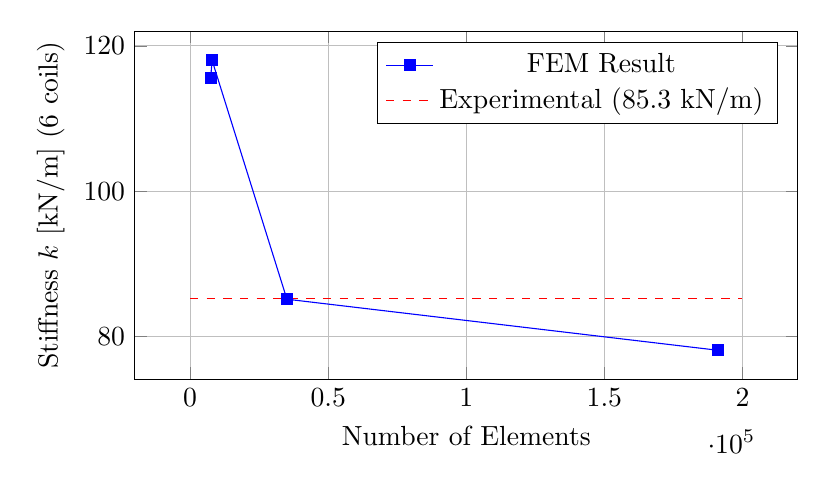
\begin{tikzpicture}
        \begin{axis}[
            width=10cm, height=6cm,
            xlabel={Number of Elements},
            ylabel={Stiffness $k$ [kN/m] (6 coils)},
            grid=major,
            legend pos=north east
        ]
        \addplot[color=blue, mark=square*] coordinates {
            (7444, 115.55)
            (7965, 118.0)
            (35050, 85.16)
            (191084, 78.14)
        };
        \addlegendentry{FEM Result}
        
        \addplot[color=red, dashed, domain=0:200000] {85.3};
        \addlegendentry{Experimental (85.3 kN/m)}
        \end{axis}
    \end{tikzpicture}
    \caption{Convergence of Rear Spring stiffness.}
    \label{fig:rear_spring_convergence}
\end{figure}

\begin{table}[H]
    \centering
    \small
    \caption{Rear Spring Parameters and Results (6 total coils).}
    \label{tab:rear_spring_results}
    \begin{tabular}{lc}
        \toprule
        \textbf{Parameter} & \textbf{Value} \\
        \midrule
        Outer Diameter ($D_{ext}$) & 80 mm \\
        Wire Diameter ($d$) & 11 mm \\
        Free Length ($L_0$) & 195 mm \\
        Experimental $k$ & 85.3 kN/m \\
        \textbf{FEM Best Result (Converged)} & \textbf{78.14 kN/m} \\
        \bottomrule
    \end{tabular}
\end{table}
